\documentclass[12pt, twoside]{article}

\setlength{\parindent}{1.25cm}
\setlength{\parskip}{0.1cm}

% codificação
\usepackage[utf8]{inputenc}

% idioma
\usepackage[brazilian]{babel}

% tamanho da folha, margens
\usepackage{geometry}
\geometry{a4paper, left=15mm, right=15mm, top=20mm, bottom=20mm, footskip=15mm}

% equações
\usepackage{amsmath}


% gráficos e flutuantes
\usepackage{float}
\usepackage{graphicx}
\usepackage{caption}

\usepackage{booktabs}

% sistema internacional de medidas
\usepackage{siunitx}

% url 
\usepackage{url}

% tabelas
\usepackage[table]{xcolor}
\usepackage{array}
\newcolumntype{P}[1]{>{\centering\arraybackslash}p{#1}}
\newcolumntype{M}[1]{>{\centering\arraybackslash}m{#1}}
\newcolumntype{L}[1]{>{\centering\arraybackslash}l{#1}}
\renewcommand{\arraystretch}{1.25}


\usepackage{circuitikz}
\usetikzlibrary{calc}
\usepackage{xcolor}

\makeatletter
\@ifpackageloaded{xcolor}{%
  \expandafter\definecolor{red}{rgb}{1,0,0}% redefining red color
}{}
\makeatother

% identação 
\usepackage{indentfirst}


% deixando os titulos das secoes em romanos
\renewcommand{\thesection}{\Roman{section}} 
\renewcommand{\thesubsection}{\thesection.\Roman{subsection}}

% espaçamento
\usepackage{setspace}
\renewcommand{\baselinestretch}{1.15} 
\setlength{\textfloatsep}{10pt plus 1.0pt minus 2.0pt}

\setlength{\columnsep}{1cm}

\usepackage{etoolbox}

\BeforeBeginEnvironment{figure}{\vskip2ex}
\AfterEndEnvironment{figure}{\vskip2ex}





\usepackage{lipsum}

% costumizações head/foot
\usepackage{fancyhdr}
% footer
\fancypagestyle{plain}{% <==============================================
\fancyhead{} % clear all header fields
\fancyhead[LO,LE]{\codigoturma}
\fancyhead[RO,RE]{\nomedisciplina}
\renewcommand{\headrulewidth}{0pt}
\fancyfoot{} 
\fancyfoot[R]{\thepage}
}

\fancypagestyle{titlepage}{% <==========================================
\fancyhead{} % clear all header fields
\fancyhead[LO,LE]{\codigoturma}
\fancyhead[RO,RE]{\nomedisciplina}
\renewcommand{\headrulewidth}{0pt}
\fancyfoot{} 
\fancyfoot[R]{\thepage}
  
}


\fancypagestyle{fancy}{% <==============================================
\fancyhead{} % clear all header fields
\fancyhead[LO,LE]{\codigoturma}
\fancyhead[RO,LE]{\nomedisciplina}
\fancyfoot{} % clear all footer fields
\renewcommand{\footrulewidth}{0.4pt}
\fancyfoot[RE,RO]{\thepage}
\fancyfoot[LO,LE]{\codigopratica}
\fancyfoot[CO,CE]{}
}

\usepackage{siunitx}

\usepackage{gensymb}

\setlength{\headheight}{15pt}


% informações da turma
\newcommand{\codigoturma}{T7600109-2024 -13}
\newcommand{\nomedisciplina}{Laboratório de Física Geral I}

% informações da prática
\newcommand{\codigopratica}{Prática 6}
\newcommand{\infopratica}{Colisões unidimensionais}

% informações do grupo
\newcommand{\alunoA}{Bruno Figueiredo Lima}
\newcommand{\nUSPalunoA}{14562383}

\newcommand{\alunoB}{Gabriel Antunes Afonso de Araujo}
\newcommand{\nUSPalunoB}{14571077}

\newcommand{\alunoC}{Ayrton da Costa Ganem Filho}
\newcommand{\nUSPalunoC}{14560190}

% data de entrega
\newcommand{\dataentrega}{18/06/2024}
\date{}

\begin{document}

\title{\vspace{-1cm} \bfseries 
\codigopratica: \infopratica}

\thispagestyle{titlepage}

\author{%
  \begin{minipage}[t]{.05\linewidth}
	\hfill
  \end{minipage}	
  \begin{minipage}[t]{.55\linewidth}
    \begin{tabular}{|p{7cm} | p{2.25cm} |}
    \hline
\rowcolor{gray!30}
    Nome &  NUSP \\
    \hline
    \rowcolor{white}
    \alunoA & \nUSPalunoA \\ \hline
    \alunoB & \nUSPalunoB \\ \hline
    \alunoC & \nUSPalunoC \\ \hline
    \end{tabular}
  \end{minipage}
  \hfill
  \begin{minipage}[t]{.35\linewidth}
  \begin{center}
  	Data de entrega: \\
	\dataentrega
\end{center}
  \end{minipage}
\vspace{0.5cm}
}	

\maketitle
\pagestyle{fancy}




\section{Objetivos}


    Essa prática tem por objetivo estudar a colisão unidimensional de um sistema composto por dois carrinhos, desconsiderando o atrito, no qual atuarão o momento linear e a energia cinética. Esses cálculos e determinações serão para dois referenciais: o laboratório e o centro de massa do sistema de partículas. Por meio do cálculo da velocidade das partículas, se calculará o momento linear e a energia cinética, para, a partir disso, determinar se o tipo de colisão foi plástica ou elástica.


\section{Introdução}


De acordo com a segunda lei de newton, força resultante de um corpo é definida como:
\begin{equation}
\label{Intro_segunda_lei_newton}
\vec{F} = m\vec{a},
\end{equation}

Para estudar as colisões unidimensionais de um sistema de partículas, precisamos entender o conceito de quantidade de movimento. A quantidade de movimento linear mede a dificuldade em que uma força tem de mudar o estado de movimento de um corpo. Ela pode ser definida como.

\begin{equation}
\label{eq:Quantidade_de_movimento}
\vec{p} = m\vec{v},
\end{equation}
Sendo assim, como $a = \frac{d\vec{v}}{dt}$, substituindo essa igualdade na equação $\ref{Intro_segunda_lei_newton}$, temos que:

\begin{equation}
\label{Intro_variacao_movimento}
\vec{F} = \frac{d\vec{p}}{dt},
\end{equation}
Dessa forma, a taxa de variação da quantidade de movimento de um corpo é a força resultante aplicada sobre ele. Sendo assim, se não há força resultante no corpo, isto é, ele permanece em seu estado de movimento, a taxa de variação da quantidade de movimento é zero. Portanto, quando a força resultante é zero em um corpo, este não muda sua quantidade de movimento, a qual permanece constante.
Sendo assim, abrangendo esse conceito para um sistema de partículas, temos que a quantidade de movimento é a soma das quantidades de movimento de cada corpo, ou seja, para um sistema de duas partículas, temos:

\begin{equation}
\label{eq:Quantidade_de_movimento_sistema}
\vec{P} = m_1\vec{v}_1 + m_2\vec{v}_2,
\end{equation}
Sendo que as forças externas atuantes no sistema de partícula é a própria variação de $\vec{P}$ ao longo do tempo.

\subsection{Colisões entre duas partículas: impulso e força média}


Em uma colisão, qualquer que seja ela, tem que a quantidade de movimento do sistema de partículas se conserva. Isso pois qualquer colisão unidimensional, durante a colisão, realiza um par de forças de ação e reação em cada partícula, o que faz com que não haja forças externas ao movimento, já que as forças internas se cancelam analisando o sistema como todo, sendo assim, de acordo com a equação $\ref{Intro_variacao_movimento}$ aplicada sobre sistemas de partículas, a quantidade de movimento se mantém. Assim:

\begin{equation}
\vec{P} = \vec{p}_{corpo 1} + \vec{p}_{corpo 2} = \text{constante}
\end{equation}

\begin{figure}[h!]
\centering
\caption{Exemplo ilustrativo relacionado ao par de forças de ação e reação durante uma colisão}
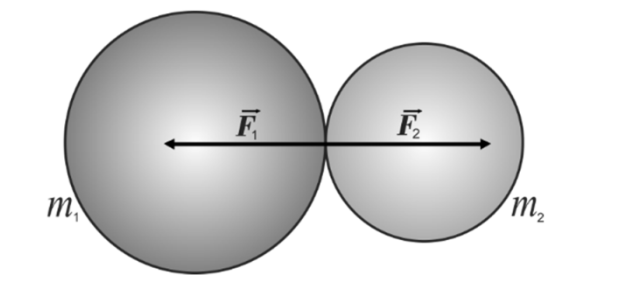
\includegraphics[width=0.5\textwidth]{introducao_impacto.png}
\caption*{Fonte: Schneider(2017)}
\label{fig:exemplo1}
\end{figure}

Impulso é uma definição que quantifica a mudança da quantidade de movimento e pode ser definida como a variação da quantidade de movimento. Sendo assim:

\begin{equation}
\label{eq:Impulso_variacao_quantidade_movimento}
I = \Delta \vec{p} = \vec{p}_{f} - \vec{p}_{i},
\end{equation}
Sendo $\vec{p}_{f}$ a quantidade de movimento final e $\vec{p}_{i}$ a quantidade de movimento inicial. Assim, conforme discutido anteriormente, para um sistema de partículas sem forças externas atuantes, o impulso é zero. Logo:

\begin{equation}
I_{\text{total}} = 0 \implies I_1 = -I_2,
\end{equation}

Dessa forma, como a força durante a colisão de partículas não é uma força constante em relação ao tempo, para calcular a variação da quantidade de movimento, ou seja, o impulso, podemos integrar a equação $\ref{Intro_variacao_movimento}$ em relação ao tempo, obtendo a seguinte relação:
\begin{equation}
\int_{t_i}^{t_f} \vec{F}\, dt = \Delta \vec{p},
\end{equation}
Sendo assim, finalmente, o impulso pode ser definido como:
\begin{equation}
I = \int_{t_i}^{t_f} \vec{F}\, dt,
\end{equation}

\begin{figure}[h!]
\centering
\caption{Representação esquemática da variação da força de contato durante uma colisão.}
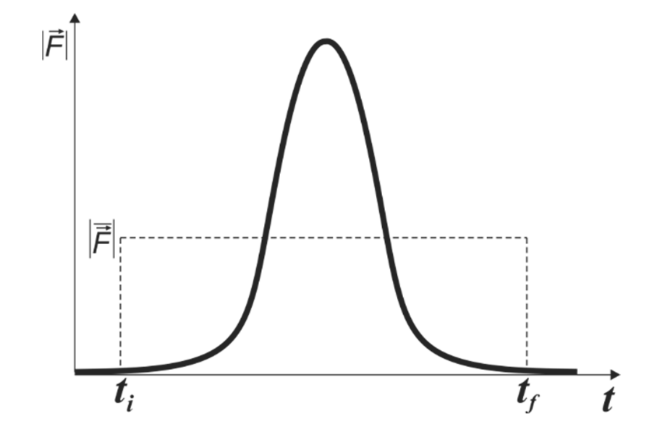
\includegraphics[width=0.5\textwidth]{introducao_grafico.png}
\caption*{Fonte: Schneider(2017)}
\label{fig:colisao}
\end{figure}

A integral de uma função pode ser interpretada, matematicamente, como a área sobre um gráfico para um determinado intervalo real. Sendo assim, para facilitar os cálculos, utilizamos uma força média denotada por $\vec{F}_{media}$ que é uma força constante imaginária sobre um corpo que possui a mesma área embaixo da curva que a função da força em relação ao tempo real. Sendo assim, a área sobre o gráfico, ou seja, o impulso, pode ser facilmente calculado pela fórmula:

\begin{equation}
\label{eq:Impulso}
I = \vec{F}_{\text{média}} \Delta t,
\end{equation}
Essa força, que é fundamental para estudar colisões, já que se torna inviável medir experimentalmente uma força como mostrada no gráfico da figura $\ref{fig:colisao}$, pode ser calculada como:
\begin{equation}
\label{eq:Forca_media}
\vec{F}_{\text{média}} = \frac{I}{\Delta t},
\end{equation}

\subsection{Velocidades e referenciais}
\label{referencial}

Para o estudo de colisões unidimensionais em um sistema de partícula, é muito importante se ter em mente o conceito de centro de massa para um dado referencial em repouso. O centro de massa é um ponto imaginário que concentra toda a massa do sistema. Sendo assim, a velocidade do centro de massa depende das velocidades e massas de cada partícula. Para um caso de um sistema com dois blocos com velocidades $\vec{v_1}$ e $\vec{v_2}$ e massas $m_1$ e $m_2$, a velocidade do centro de massa pode ser calculada como:
\begin{equation}
\label{eq:Velcidade_centro_de_massa}
\vec{v}_{cm} = \frac{m_1\vec{v}_1 + m_2\vec{v}_2}{m_1 + m_2},
\end{equation}
Sendo a quantidade de movimento do centro de massa dado por:
\begin{equation}
\label{eq:Quantidade_de_movimento_centro_de_massa}
\vec{P} = (m_1 + m_2) \vec{v}_{cm},
\end{equation}
Dessa forma, pode-se concluir que se a resultante de forças externas é nula, o centro de massa possui velocidade constante. Além disso, se as quantidades de movimento de dois corpos em sentidos opostos são iguais, o centro de massa do sistema permanece em repouso. 
Por fim, caso um observador estivesse viajando na mesma velocidade, direção e sentido do centro de massa do sistema de partículas, as velocidades medidas seriam diferentes. A relação entre as velocidades pode ser dada a partir da transformação de Galileu, isto é, a velocidade $\vec{u}$ medida por quem viaja junto com o centro de massa,  é a diferença entre a velocidade medida por quem está num referencial do chão do laboratório menos $\vec{v_{cm}}$.

\subsection{Energia cinética em sistemas de partículas em colisão}

Para estudo de movimentos com colisão unidimensional, é importante estudar como a energia mecânica se comporta durante o movimento, seja antes ou depois da colisão. É importante ressaltar que, caso a colisão não deforme nenhum dos corpos nem gere nenhum aquecimento, ou seja, a energia mecânica não é transformada em outro tipo de energia, se pode concluir que a soma da energia cinética mais a energia potencial se torna constante, ou seja, a energia mecânica se conserva. Portanto, a energia cinética de um movimento irá se conservar a depender da natureza dos corpos. Para classificar os choques e indicar se a energia cinética é diminuída ou conservada, é importante definir o coeficiente de restituição para quantificar essa perda de energia cinética, que relaciona as velocidades relativas entre os corpos antes e depois da colisão e pode ser calculada por:

\begin{equation}
\label{eq:Coeficiente_de_restituicao_elastica}
e = \frac{|\vec{v}_{2f} - \vec{v}_{1f}|}{|\vec{v}_{1i} - \vec{v}_{2i}|},
\end{equation}
Sendo $\vec{v}$ a velocidade relativa que pode ser medida pela diferença entre a velocidade do corpo 2 e a velocidade do corpo 1. 

As colisões podem ser classificadas conforme a tabela abaixo:


\begin{table}[h!]
\centering
\caption{Classificação dos tipos de colisão em função da variação da energia cinética total e comportamentos do coeficiente de restituição e da quantidade de movimento total.}
\begin{tabular}{|m{4cm}|m{4cm}|m{4cm}|m{4cm}|}
\hline
\textbf{Colisão} & \textbf{Energia cinética} & \textbf{Coeficiente de restituição} & \textbf{Quantidade de movimento} \\ 
\hline
Perfeitamente elástica & Conserva & \(e = 1\) & Conserva \\ 
\hline
Parcialmente elástica & Diminui & \(0 < e < 1\) & Conserva \\ 
\hline
Perfeitamente plástica & Máxima diminuição & \(e = 0\) & Conserva \\ 
\hline
\end{tabular}
\caption*{Elaborado pelos autores}
\label{table:colisao}
\end{table}








\section{Métodos}

\subsection{Propagação de erro}

Para realizar medições de medidas diretas, todos os instrumentos utilizados possuem erros de medidas. Dessa forma, para realizar cálculos com equações que utilizam medições diretas, é necessário realizar uma propagação do erro das medidas calculadas.
Segundo Schneider (2017), a fórmula para o cálculo da propagação de um valor $f$ é dado por:
            \begin{equation}
                \label{eq:propagacao_de_erro} 
                \Delta f = \left| \frac{\partial f}{\partial x} \right| \Delta x + \left| \frac{\partial f}{\partial y} \right| \Delta y,
	    \end{equation}
De modo geral, podemos definir como uma função de três variáveis da seguinte maneira:
           \begin{equation}
    \label{eq:propagacao_de_erro_3}
    \Delta f = \left| \frac{\partial f}{\partial x} \right| \Delta x + \left| \frac{\partial f}{\partial y} \right| \Delta y + \left| \frac{\partial f}{\partial z} \right| \Delta z,
\end{equation}

\subsection{Comparando os resultados}
\label{Analise_de_eq}

Após calculados os resultados da gravidade com suas respectivas incertezas, $(x_1 \pm \sigma_1)$ e ${(x_2 \pm \sigma_2)}$, relativos às medidas da gravidade nos dois experimentos. Esses resultados são equivalente se, e somente se, satisfazer a seguinte desigualdade:
 
		\begin{equation}
        \label{eq:comparacao equivalente}
                |x_1 - x_2| < 2(\sigma_1 + \sigma_2),
	    \end{equation}
     
    Entretanto, dois resultados são ditos não equivalentes se, e somente se:
    
		\begin{equation}
            \label{eq:comparacao nao equivalente} 
                |x_1 - x_2| > 3(\sigma_1 + \sigma_2),
	    \end{equation}
     
    Caso o resultado experimental seja da forma $2(\sigma_1 + \sigma_2) < |x_1 - x_2| < 3(\sigma_1 + \sigma_2)$, não é possível afirmar a equivalência dos resultados obtidos.

\section{Materiais}


\subsection{Instrumentos}
    Nesse experimento, será utilizado um trilho de ar, acoplado com laser e um carrinho. Esse suporte possibilita que o carrinho se mova sobre o trilho com um atrito reduzido. Os instrumentos podem ser vistos abaixo:

    \begin{figure}[h!]
\centering
\caption{Trilho de ar para estudar colisões unidimensionais. O carrinho 1 é incidente e o carrinho 2 está em repouso inicialmente, sendo a colisão aproximadamente elastica, devido às disposições das molas}
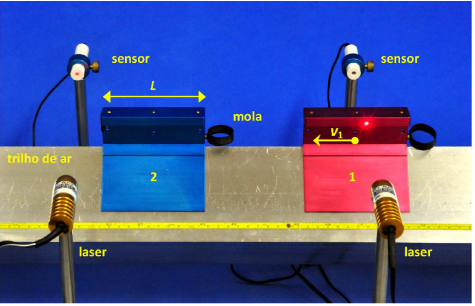
\includegraphics[width=0.5\textwidth]{Materiais_trilho.png}
\caption*{Fonte: Schneider(2017)}
\label{fig:exemplo}
\end{figure}
        



    \subsection{Medidas diretas}

    \begin{itemize}
        \item  Tempo de passagem do carrinho pelo laser
        \end{itemize}
Para calcular o tempo em que o laser fica obstruído devido à passagem do carrinho, será utilizado um cronômetro que mede o tempo em que o carrinho passou pelo laser e sua precisão é de 0,001 segundo.
        
    \begin{itemize}
        \item  Massa dos carrinhos
        \end{itemize}
Para calcular a massa dos carrinhos juntos ou separados, será usada uma balança, sendo sua precisão de $10^{-5}$ Kg.

\begin{itemize}
        \item  Comprimento do carrinho
        \end{itemize}

        Será utilizado uma régua para medir o comprimento do carrinho, sendo sua precisão de $10^{-3}$ metros. 

    \subsection{Medidas indiretas}

    
    \begin{itemize}
        \item Velocidade delta l delta t dos carrinhos
        \end{itemize}

Dado o comprimento do carrinho, para calcular a velocidade em que ele passa pelo laser, fazemos uma razão entre os valores do comprimento do carrinho e o tempo medido pelo laser. Assim, temos:
        \begin{equation}
        \label{Materiais_Equacao_velocidade}
            v = \frac{L}{t}
        \end{equation}
        Em que seu erro é dado por:

        \begin{equation}
        \label{Materiais_Erro_Equacao_velocidade}
            \delta v = \frac{\delta L t + \delta t L}{t^2}
        \end{equation}
        

        \begin{itemize}
        \item Quantidade de movimento
        \end{itemize}

Dado a medida da velocidade calculada anteriormente e a medida direta da massa, temos que a quantidade de movimento é:
        \begin{equation}
        \label{Materiais_equacao_quantidade_de_movimento}
            \vec{P} = m\cdot \vec{v}
        \end{equation}
Seu erro é calculado por:

\begin{equation}
        \label{Materiais_erro_equacao_quantidade_de_movimento}
            \delta{P} = \delta{m}v + \delta{v}m
        \end{equation}
E sua variação percentual por:

        \begin{equation}
        \label{Materiais_percentual1_quantidade_de_movimento}
            \Delta{P}(\%) = 100 . \frac{|P_i - P_f|}{P_i}
        \end{equation}
Onde seu erro é dado por:
\begin{equation}
        \label{Materiais_erro_percentual1_quantidade_de_movimento}
            \delta\Delta{P}(\%) = 100 . \frac{(\delta P_i + \delta P_f)P_i + \delta P_i(|P_i - P_f|)}{P_i^2}
        \end{equation}

Porém, caso a quantidade de movimento inicial seja nula, a equação anterior resultaria em uma indeterminação. Para isso, usamos a seguinte variação:

        \begin{equation}
            \label{Materiais_percentual2_quantidade_de_movimento}
            \Delta{P}(\%) = |P_f - P_i| 
        \end{equation}
        %% Não tenho certeza disso... Vou procurar a fórmula e acertar mais tarde

        \begin{itemize}
        \item Impulso
        \end{itemize}

Tendo a quantidade de movimento, o impulso é calculado como a variação da quantidade de movimento. Sendo assim, temos:
        \begin{equation}
        \label{Materiais_equacao_impulso}
            \vec{I} = \Delta \vec{P} = \vec{P}_i - \vec{P}_f
        \end{equation}
O erro do impulso é dado por:
\begin{equation}
        \label{Materiais_erro_equacao_impulso}
            \delta{I} =\delta{P}_i + \delta{P}_f
        \end{equation}


        \begin{itemize}
        \item Energia cinética
        \end{itemize}
A energia cinética é uma energia que depende da velocidade de um corpo e de sua massa. Pode ser calculada por:
        \begin{equation}
        \label{Materiais_energia_cinetica}
            E_c = \frac{1}{2}\cdot mv^2
        \end{equation}
Seu erro é dado por:

\begin{equation}
        \label{Materiais_erro_energia_cinetica}
            \delta E_c = \frac{(\delta m) v^2 + 2mv (\delta v)}{2}
        \end{equation}
E sua variação percentual por:

        \begin{equation}
        \label{Materiais_percentual1_energia_cinetica}
            \Delta{E_c}(\%) = 100 . \frac{|E_{ci} - E_{cf}|}{E_{ci}}
        \end{equation}

    Porém, asssim como para o percentual da qantidade de movimento, uma energia cinética inicial nula também resultaria em uma indeterminação. Por isso, aplicamos a seguinte variação para esses casos:

        \begin{equation}
            \label{Materiais_percentual2_energia_cinetica}
            \Delta{E_c} = |E_{cf} - E_{ci}|
        \end{equation}
Seu erro é dado por:
\begin{equation}
        \label{Materiais_erro_percentual1_energia_cinetica}
            \delta\Delta{E_c}(\%) = 100 . \frac{(\delta E_{ci} + \delta E_{cf})E_{ci} + \delta E_{ci}(|E_{ci} - E_{cf}|)}{E_{ci}^2}
        \end{equation}


        \begin{itemize}
        \item Coeficiente de restituição
        \end{itemize}
O coeficiente de restituição depende da velocidade relativa de um determinado corpo. Essa velocidade relativa pode ser calculada por:
        \begin{equation}
        \label{Materiais_velocidade_relativa}
            \vec{V_r} = \vec{v_2}-\vec{v_1}
        \end{equation}
Sendo $\vec{v_2}$ e $\vec{v_1}$ as velocidades dos corpos em análise.
Sendo assim, tendo as velocidades relativas, o coeficiente de restituição pode ser calculado por:
        \begin{equation}
        \label{Materiais_coeficiente_de_restituicao}
            e = \frac{|\vec{V_{rf}}|}{|\vec{V_{ri}}|}
        \end{equation}
E seu erro é dado por:

        \begin{equation}
        \label{Materiais_erro_coeficiente_de_restituicao}
            e = \frac{\delta (\vec{|V_{rf}|})|\vec{V_{ri}}| + |\vec{V_{rf}}| \delta (\vec{|V_{ri}|})}{\vec{|V_{ri}}|^2}
        \end{equation}

        \begin{itemize}
        \item Força de contato
        \end{itemize}

Conforme discutido anteriormente, é necessário determinar uma força média no experimento. A força média é determinada com um $\Delta t$ fixo e pode ser determinada a partir do impulso e do tempo da seguinte forma:
        \begin{equation}
        \label{Materiais_forca_de_Contato}
            \vec{F} = \frac{\vec{I}}{\Delta t}
        \end{equation}
Sendo seu erro dado por:

\begin{equation}
        \label{Materiais_erro_forca_de_Contato}
            \vec{F} = \frac{\delta (\vec{I}) \Delta t + \vec{I} \delta (\Delta t)}{\Delta t^2}
        \end{equation}


        \begin{itemize}
        \item Velocidade de centro de massa
        \end{itemize}

É definida como a velocidade do ponto que representa a média ponderada das posições dos dois corpos, levando em conta suas massas.  Nessa relação, $m1$ e $m2$ representam a massa do objeto 1 e do objeto 2, respectivamente, e suas respectivas velocidades são representadas por $\vec{v_1}$ e $\vec{v_2}$.

 
        \begin{equation}
        \label{Materiais_velocidade_Centro_de_massa}
            \vec{V_{CM}} = \frac{m_1\cdot \vec{v_1} + m_2\cdot \vec{v_2}}{m_1+m_2}
        \end{equation}

Sendo seu erro dado pela soma de $\delta(\vec{V_{CM,i}})$ com $\delta(\vec{V_{CM,f}})$, sendo esses determinados por:
\begin{equation}
\label{Materiais_erro_velocidade_Centro_de_massa_simplificada_1}
\delta(\vec{V_{CM,i}}) = \sqrt{ \left( \frac{m_2 \vec{v_{1,i}}}{(m_1 + m_2)^2} \delta(m_1) \right)^2 + \left( -\frac{m_1 \vec{v_{1,i}}}{(m_1 + m_2)^2} \delta(m_2) \right)^2 + \left( \frac{m_1}{m_1 + m_2} \delta(\vec{v_{1,i}}) \right)^2 }
\end{equation}
\begin{equation}
\label{Materiais_erro_velocidade_Centro_de_massa_final_2}
\delta(\vec{V_{CM,f}}) = \sqrt{ \left( -\frac{m_2 \vec{v_{2,f}}}{(m_1 + m_2)^2} \delta(m_1) \right)^2 + \left( \frac{m_1 \vec{v_{2,f}}}{(m_1 + m_2)^2} \delta(m_2) \right)^2 + \left( \frac{m_2}{m_1 + m_2} \delta(\vec{v_{2,f}}) \right)^2 }
\end{equation}
%%% ERRROOOO



\section{Resultados}
\subsection{Choque elástico entre dois corpos de massas iguais com referencial no laboratório}

\subsubsection{Dados coletados para as duas colisões estudadas}
\label{DadosColetados}

    Iniciamos a prática obtendo todas as medidas diretas do sistema, que seriam necessárias para calcular sua quantidade de movimento, tipo de colisão e conservação de energia nos diversos referenciais. Primeiramente, com uma régua, medimos o comprimento dos corpos envolvidos na colisão e, para a colisão plástica, o seu comprimento em conjunto, obtendo: $l_1 = (0,105 \pm 0,001)m$, $l_2 = (0,105 \pm 0,001)m$ e $l_t = (0,212 \pm 0,001)m$. Quanto a massa dos corpos envolvidos no sistema, usamos uma balança, determinando-a para ambos separadamente e em conjunto (novamente, devido ao posterior estudo da colisão plástica), chegando a: $m_1 = (0,18000 \pm 0,00001)kg$, $m_2 = (0,18000 \pm 0,00001)kg$ e $m_t = (0,36126 \pm 0,00001)kg$.

    Posteriormente, realizamos a parte prática do experimento, usando o cronômetro digital para determinar o tempo  antes e depois da colisão. Para a colisão elástica, obtivemos $t_{e1} = (0,105 \pm 0,001)s$ e $t_{e2} = (0,107 \pm 0,001)s$, enquanto para a colisão plástica: $t_{p1} = (0,103 \pm 0,001)s$ e $t_{p2} = (0,413 \pm 0,001)s$.

    Ademais, vale citar que todos os resultados obtidos posteriormente consistiram em medidas indiretas, para as quais propagamos as incertezas utilizando a equação (\ref{eq:propagacao_de_erro}).

\subsubsection{Cálculo das velocidades e quantidades de movimento do sistema}
\label{velocidadesCalculadas1}

    Com todas as medidas diretas necessárias em mãos, passamos a calcular as grandezas físicas relacionadas ao movimento do sistema. Usando as medidas de comprimento e os tempos obtidos durante a colisão elástica, e aplicando as equações (\ref{Materiais_Equacao_velocidade}) e (\ref{Materiais_Erro_Equacao_velocidade}) determinamos as velocidades inicial e final dos corpos 1 e 2, respectivamente, obtendo: $v_{1i} = (1,00 \pm 0,02)\frac{m}{s}$ e $v_{2f} = ( 0,98 \pm 0,02)\frac{m}{s}$. Vale citar, que tanto $v_{2i}$ e $v_{1f}$ equivalem a $0\frac{m}{s}$, pois os corpos se encontram em repouso no sistema nesses respectivos instantes.

    Com as velocidades determinadas, aplicamos a equação (\ref{Materiais_equacao_quantidade_de_movimento}) e novamente propagamos o erro com (\ref{Materiais_erro_equacao_quantidade_de_movimento}) para obter as quantidades de movimento de ambos os códigos antes da colisão e depois da colisão. Para antes da colisão, obtivemos (para os corpos 1 e 2 respectivamente): $P_{1i} = (0,180 \pm 0,004)kg\frac{m}{s}$ e $P_{2i} = 0 kg\frac{m}{s}$, enquanto para o fim $P_{1f} = 0 kg\frac{m}{s}$ e $P_{2f} = (0,177 \pm 0,004) kg\frac{m}{s}$.

\subsubsection{Variação percentual da quantidade de movimento do sistema e discussão}

    Usando a equação (\ref{Materiais_percentual1_quantidade_de_movimento}), determinamos a variação percentual da quantidade de movimento para essa colisão, chegando a $\Delta P(\%) = (2 \pm 4)\%$. Considerando o erro, podemos chegar ao seguinte intervalo para o percentual provável: $-2 < \Delta P(\%) < 6$ que, por conter 0, nos permite afirmar que a quantidade de movimento do sistema se conserva.

\subsubsection{Impulso sofrido pelos corpos e discussão}

    Para o cálculo do impulso nos corpos utilizamos a equação (\ref{Materiais_equacao_impulso}), enquanto o impulso total foi obtido somando os dois resultados anteriores. Então, chegamos aos valores: $I_1 = (-0,180 \pm 0,004)N.s$,  $I_2 = (0,177 \pm 0,004)N.s$ e $I_f = (-0,003 \pm 0,008)N.s$, os quais correspondem ao impulso dos corpos 1, 2 e o impulso total do sistema, respectivamente. Além disso, o impulso total obtido se aproxima de zero (especialmente se considerarmos o erro), indicando que a quantidade de movimento se conservou, como era esperado pelo percentual obtido anteriormente.


\subsubsection{Cálculo das energias cinéticas do sistema e do coeficiente de restituição elástica}

    Contudo, a fim de determinar se a colisão efetivamente foi elástica, ainda havia outras grandezas que precisavam ser analisadas e discutidas. 

    Primeiramente, com a equação (\ref{Materiais_energia_cinetica}) calculamos as energias cinéticas do sistema antes e após a colisão, obtendo, respectivamente: $Ec_{i} = (0,090 \pm 0,004)J$ e $Ec_{f} = (0,086 \pm 0,004)J$. Além disso, ao aplicar a equação (\ref{Materiais_percentual1_energia_cinetica}), determinamos a variação percentual dessa energia como $\Delta Ec(\%) = (5 \pm 9)\%$ que, considerando o intervalo para o percentual provável; isto é: $-4 < \Delta Ec(\%) < 14$ contém $0$, indicando que a energia cinética se conservou (Um forte indicativo para a colisão ser elástica).

    Por fim, calculamos o coeficiente de restituição elástica com a equação (\ref{Materiais_coeficiente_de_restituicao}), chegando a e = $0,98 \pm 0,08$ que, é extremamente próximo de 1 (especialmente quando leva em conta a sua incerteza), classificando a colisão como elástica, assim como o esperado.

\subsubsection{Força média para os corpos durante a colisão}

    Afinal, usamos a equação (\ref{Materiais_forca_de_Contato}) para determinar a força média exercida em ambos os corpos durante a colisão, adotando o intervalo de tempo do choque como $\Delta t = 0,001 s$, chegando em $Fm_1 = (-180 \pm 4) N$ e $Fm_2 = (177 \pm 4)N$.
    

\subsection{Choque elástico entre dois corpos de massas iguais com referencial no centro de massa}

\subsubsection{Cálculo da velocidade do centro de massa antes e após a colisão}

    Antes de tudo, vale citar que os tópicos a seguir, ainda fazem parte da primeira parte do experimento. Porém, os mesmo cálculos foram feitos para o referencial do centro de massa dos corpos envolvidos. Assim, as velocidades relativas mudaram, impactando diretamente os valores das outras grandezas, mas as equações utilizadas para a maioria das medidas indiretas são as mesmas(sendo elas as quantidades de movimento, impulsos, energias cinéticas e o coeficiente de restituição).

    Em um primeiro momento, determinamos as velocidades do centro de massa para antes e depois da colisão usando a equação (\ref{Materiais_velocidade_Centro_de_massa}), obtendo, respectivamente, $vcm_{i} = (0,50 \pm 0,01)\frac{m}{s}$ e $vcm_{f} = (0,49 \pm 0,01)\frac{m}{s}$. Podemos observar que esses resultados são compatíveis com a conservação da quantidade de movimento no sistema, pois a velocidade do centro de massa (a qual considera o movimento de ambos corpos envolvidos) praticamente não sofreu alteração após a colisão.
    
\subsubsection{Cálculo das velocidades e quantidades de movimento do sistema}
\label{novasVelocidades}

    A partir das velocidades do centro de massa, podemos recalcular as velocidades dos corpos no sistema antes e depois da colisão, passando a lançar um novo olhar ao sistema, por analisá-lo pelo referencial do centro de massa. Dessa forma, aplicando a equação de velocidade relativa (\ref{Materiais_velocidade_relativa}), obtemos como velocidades relativas iniciais e finais dos corpos 1 e 2, respectivamente: $u_{1i} = (0,50 \pm 0,03)\frac{m}{s}$, $u_{2i} = (-0,50 \pm 0,03)\frac{m}{s}$, $u_{1f} = (-0,49 \pm 0,03)\frac{m}{s}$ e $u_{1f} = (0,49 \pm 0,03)\frac{m}{s}$.

    Ademais, ao recalcular as quantidades de movimento iniciais e finais dos corpos 1 e 2 com essas velocidades, chegamos em: $P_{1i} = (0,090 \pm 0,005) kg\frac{m}{s}$, $P_{2i} = (-0,090 \pm 0,005) kg\frac{m}{s}$, $P_{1f} = (0,088 \pm 0,005) kg\frac{m}{s}$ e $P_{1i} = (-0,088 \pm 0,005) kg\frac{m}{s}$. 

\subsubsection{Variação percentual da quantidade de movimento do sistema e discussão}

    Com as quantidades de movimento em relação ao centro de massa, recalculamos o seu percentual, obtendo $\Delta P(\%) = (0,00 \pm 0,05)\%$. O que nos permite afirmar que a quantidade de movimento do sistema se conserva.

    É necessário citar que, para este caso específico, a equação (\ref{Materiais_percentual1_quantidade_de_movimento}) acarretaria em uma indeterminação, uma vez que a somatória das quantidades de movimento iniciais e finais equivalem a $0$. Por isso, foi aplicada a equação (\ref{Materiais_percentual2_quantidade_de_movimento}).

\subsubsection{Impulso sofrido pelos corpos e discussão}

    Utilizando novamente as quantidades de movimento em relação ao centro de massa, recalculamos os impulsos dos corpos 1 e 2, bem como o impulso total do sistema, obtendo, respectivamente: $I_1 = (0,00 \pm 0,01)N.s$,  $I_2 = (0,00 \pm 0,01)N.s$ e $I_f = (0,00 \pm 0,02)N.s$, sendo que este resultado também contribui para a afirmação de que a quantidade de movimento está se conservando, dado que o impulso total equivale a zero.

\subsubsection{Cálculo das energias cinéticas do sistema e do coeficiente de restituição elástica}

    Concomitantemente aos cálculos para o referencial do laboratório, calculamos as energias cinéticas, determinamos sua variação percentual e obtivemos o coeficiente de restituição para enfim determinar se a colisão do sistema foi elástica.
    Quanto às energias, obtivemos: $Ec_{i} = (0,000 \pm 0,003)J$, $Ec_{f} = (0,000 \pm 0,003)J$. Porém, esse resultado também faria com que o cálculo da sua variação acarretasse em uma indeterminação, por isso, utilizamos a equação (\ref{Materiais_percentual2_energia_cinetica}), chegando em $\Delta Ec(\%) = (0,000 \pm 0,006)\%$, o que indica que não houve variação de energia cinética e, portanto, ela se conservou durante a colisão.

    Por fim, empregamos as velocidades relativas ao centro de massa de (\ref{novasVelocidades}) no cálculo do coeficiente de restituição elástica, obtendo: $e = (0,98 \pm 0,09)$, o qual, considerando o erro, também se aproxima de $1$, indicando, mais uma vez, a colisão como elástica.

\subsubsection{Conclusão para a compatibilidade dos resultados dos dois referenciais}

    Analisando os valores obtidos em ambos os referenciais, concluímos que os estudos tiveram resultados compatíveis, com suas variações percentuais de quantidade de movimento e impulsos finais indicando que essa quantidade de movimento se conservou, assim como a energia cinética (pelo cálculo da variação percentual das energias cinéticas), o que fortemente aponta para uma colisão elástica, que não só era esperada, como também pode ser confirmada pelos coeficientes de restituição elástica, já que ambos se aproximaram de $1$.

    Vale citar que, ao aplicar a relação (\ref{eq:comparacao equivalente}) para as variações e coeficientes de restituição, o resultado é equivalente.

    %% Acho melhor botar aquela relação para determinar se os resultados com incerteza foram equivalentes. Só por garantia

\subsection{Choque plástico entre dois corpos de massas iguais}
\subsubsection{Mudanças nas medidas usadas para o choque plástico}

    De início, é importante ressaltar que a segunda parte do experimento, ao apresentar um choque plástico entre os corpos, na qual eles passam a se locomover em conjunto, levou a necessidade de calcular a somatória de suas massas, sendo que estas foram medidas diretamente e expressas na seção \ref{DadosColetados}. Além disso, vale citar que, novamente, fomos capazes de utilizar as mesmas equações para o cálculo das medidas indiretas, seguindo um passo a passo similar à primeira parte do experimento.

\subsubsection{Cálculo das velocidades e quantidades de movimento do sistema}
\label{velocidadePlastica}

    Utilizando os tempos da colisão plástica ($t_{p1}$ e $t_{p2}$), bem como os comprimentos de ambos os corpos, passamos a calcular as suas velocidades antes e após a colisão. Porém, há uma grande diferença após a colisão, se relacionarmos com os cálculos anteriores: Os corpos passaram a se mover em conjunto, podendo ser descritos como algo único e, consequentemente, tendo uma única velocidade ($v_j$). Logo, obtivemos: $v_{1ip} = (1,02 \pm 0,02)\frac{m}{s}$,  $v_{2ip} = 0\frac{m}{s}$ e $v_j = (0,513 \pm 0,004)\frac{m}{s}$.

    Ademais, usamos estes resultados para determinar as novas quantidades de movimento envolvidas no sistema antes para os corpos 1 e 2 antes da colisão, bem como para os corpos se locomovendo em conjunto após a colisão, sendo elas, respectivamente: $P_{1i} = (0,184 \pm 0,004) kg\frac{m}{s}$, $P_{2i} = 0 kg\frac{m}{s}$, $P_j = (0,185 \pm 0,001) kg\frac{m}{s}$

\subsubsection{Variação percentual da quantidade de movimento do sistema e discussão}

    Visando determinar se essa quantidade se conservou ou não, novamente efetuamos o cálculo da variação percentual da quantidade de movimento para os novos resultados obtidos (nesse caso, voltando a usar a equação (\ref{Materiais_erro_percentual1_quantidade_de_movimento})), chegando em: $\Delta P(\%) = (1 \pm 3)\%$. Considerando o erro, determinamos o intervalo para o percentual provável como $-2 < \Delta P(\%) < 4$ que, por conter $0$, nos permite afirmar que a quantidade de movimento do sistema também se conservou para essa nova colisão.

\subsubsection{Impulso sofrido pelos corpos e discussão}

    Utilizando mais uma vez as novas quantidades de movimento em relação ao centro de massa, recalculamos os impulsos dos corpos 1 e 2, bem como o impulso total do sistema, obtendo, respectivamente: $I_1 = (-0,091 \pm 0,004)N.s$,  $I_2 = (0,0923 \pm 0,0007)N.s$ e $I_f = (0,001 \pm 0,005)N.s$, sendo que este resultado novamente contribui para a afirmação de que a quantidade de movimento está se conservando, dado que o impulso total (quando considerada a incerteza) se aproxima de $0$.

    Porém, vale citar que houve a necessidade de manipular as equações de impulso: (\ref{Materiais_equacao_impulso}) e (\ref{Materiais_erro_equacao_impulso}), só considerando a massa do respectivo corpo estudado para a quantidade de movimento final (mesmo estando em conjunto com o outro corpo).

\subsubsection{Cálculo das energias cinéticas do sistema e do coeficiente de restituição elástica} %% Não esquecer das conclusões nessa parte, camarada!

    Por fim, terminamos o experimento calculando e analisando as grandezas necessárias para determinar o tipo de colisão.
    
    De início, empregamos as velocidades e massas obtidas ao longo do experimento para essa colisão ($v_{1ip}$, $v_{2ip}$, $v_j$, $m_1$ e $m_t$) no cálculo das energias cinéticas antes e após ela, obtendo, respectivamente: $Ec_{i} = (0,09 \pm 0,04)J$, $Ec_{f} = (0,04754 \pm 0,00007)J$. Assim, usamos esses valores para determinar a variação percentual da energia cinética, chegando em: $\Delta Ec(\%) = (47,2 \pm 0,7)\%$, o qual pelo intervalo da incerteza percentual gerado: $46,5 \% < \Delta Ec(\%) < 47,9 \%$, mostra que ela se aproximou do esperado para esse tipo de colisão, pois ao invés de se conservar, houve uma perda considerável.

    Além disso, aplicamos as velocidades encontradas nesse sistema ($v_{1ip}$, $v_{2ip}$, $v_j$) durante as colisões para o cálculo do coeficiente de restituição, obtendo $e$ = $0$ (uma vez que as velocidades finais de 1 e 2 são iguais). Dessa forma, fomos capazes de concluir que a colisão é de fato plástica.

\section{Conclusões}

\subsection{Choque elástico entre dois corpos de massas iguais}

Antes de mais nada, medimos, como exposto em \ref{DadosColetados}, $m_1, m_2, l_1, l_2$, fizemos então o experimento, registrando os tempos de passagem de cada carro no laser após o choque: $t_1$ e $t_2$.

Com esses dados, calculamos então a velocidade de cada carro antes e após a colisão. Do carro 1 obtivemos então $v_{1i}$ e $v_{1f}$, e do carro 2, $v_{2i}$ e $v_{2f}$, com seus valores expostos em \ref{velocidadesCalculadas1}. Com isso, podemos calcular a quantidade de movimento de cada carro no momento final e inicial: $P_{1i} = (0,180\pm0,004)kg \frac{m}{s}, P_{2i} = 0 kg\frac{m}{s}, P_{1f} = 0 kg \frac{m}{s}, P_{2f} = (0, 177 \pm 0,004)kg \frac{m}{s}$. Logo chegamos, olhando para a quantidade de movimento do sistema como um todo, em seu momento inicial e final em, respectivamente: $P_i = (0,180\pm0,004)kg\frac{m}{s}$ e $P_f = (0,177\pm0,004)kg\frac{m}{s}$.

Após esses cálculos, podemos calcular a variação percentual dessa quantidade de movimento, chegando ao valor de $\Delta P(\%) = (2\pm4)\%$. Esse valor, como discutido, é próximo de zero, o que implica na conservação da quantidade de movimento do sistema.

Agora, usando os dados já coletados, calculamos então o impulso que atua em cada bloco: $I_1 = (-0,180\pm 0,004)N\cdot s, I_2 = (0,177\pm 0,004)N\cdot s$, obtendo $\Sigma I_i = (-0,003 \pm 0,008) N\cdot s$. Logo, pelo impulso total obtido (que é muito próximo de zero), concluímos novamente que houve conservação de quantidade de movimento do sistema.

Agora, calculamos a energia cinética e o coeficiente de restituição elástica do sistema, a fim de mostrar que, de fato, a colisão foi elástica. Para a energia cinética inicial e final obtivemos, respectivamente: $E_{c_i} = (0,090 \pm 0,004)J$ e $E_{c_f} = (0,086\pm0,004)J$. A variação percentual foi de: $\Delta E_c(\%) = (5\pm9)\%$, o que nos permite concluir que houve sim conservação de energia, já que o valor se aproxima de zero. Calculando, por fim, o coeficiente de restituição elástica, chegamos no valor $e = (0,98\pm0,08)$, o que é bem próximo de 1, o que nos permite concluir que a colisão de fato foi elástica.

Por fim, medimos a força média exercida em cada um dos corpos, adotando o tempo de contado como $\Delta t = 0,001s$. Chegamos em $F_{m_1} = (-180\pm4)N, F_{m_2}=(177\pm4)N$.

\subsubsection{Referencial centro de massa}

Primeiramente, calculamos a velocidade do centro de massa final e inicial que são, respectivamente: $vcm_i = (0,50\pm0,01)\frac{m}{s}, vcm_f = (0,49\pm0,01)\frac{m}{s}$. Vale a pena perceber o fato de que as velocidades praticamente não se alteraram, o que é compatível com uma conservação da quantidade de movimento desse sistema.

Antes de aplicar os cálculos dentro desse novo referencial, devemos utilizar o discutido em \ref{referencial} para calcularmos as novas velocidades com esse novo referencial, que foram expostas em \ref{novasVelocidades}.

Após isso, recalculamos a quantidade de movimento inicial e final para cada bloco, chegando em: $P_{1i} = (0,090\pm0,005)kg \frac{m}{s}, P_{2i} = (-0,090\pm0,005) kg\frac{m}{s}, P_{1f} = (0,088\pm0,005) kg \frac{m}{s}, P_{2f} = (-0,088\pm0,005)kg \frac{m}{s}$. Calculando novamente a variação percentual da quantidade de movimento, chegamos em: $\Delta P(\%)=(0,00\pm0,05)$, o que nos permite afirmar que a quantidade de movimento do sistema se conserva.

Calculando os impulsos em cada bloco, temos $I_1 = (0,00\pm0,01)N\cdot s, I_2 = (0,00\pm0,01)N\cdot s$. Logo $\Sigma I_i = (0,00\pm0,02)N\cdot s$. Esse resultado também nos leva a conclusão de que houve conservação da quantidade de movimento do sistema.

Calculando a energia cinética inicial e final, obtemos, respectivamente, $E_{c_i} = (0,000\pm0,003)J, E_{c_f} = (0,000\pm0,003)J$. A variação percentual é de $\Delta E_c(\%) = (0,000\pm0,006)\%$ que, juntamente com o valor calculado do coeficiente de restituição elástica $e = 0,98\pm0,09$, nos permite concluir que a colisão foi, de fato, elástica.

\subsubsection{Conclusão sobre a troca de referenciais}

Como observado, independente do referencial, chegamos a conclusão de que houve conservação da quantidade de movimento do sistema e de energia, o que nos leva a conclusão de que a colisão é elástica.

\subsection{Choque plástico entre dois corpos de massas iguais}

Vale ressaltar que, para esse choque, usaremos os mesmos blocos e, portanto, as massas são idênticas à primeira parte. Além disso, medimos a massa após a colisão (quando os blocos se unem), que é de $m_t = (0,36126\pm0,00001)kg$. Medimos, novamente o tempo em que cada objeto passa no laser, a fim de calcular a velocidade do objeto (ver \ref{velocidadePlastica}).

Após isso, calculamos a quantidade de movimento inicial do corpo 1 e inicial do corpo 2, e a final do corpo resultante do choque, obtendo respectivamente: $P_{1i} = (0,184\pm0,004)kg\frac{m}{s}, P_{2i}=0kg\frac{m}{s}, P_j=(0,185\pm0,001)kg\frac{m}{s}$. Determinando a variação percentual, obtemos $\Delta P(\%) = (1\pm3)\%$, o que nos permite afirmar que a quantidade de movimento nessa nova colisão também se conserva.

Calculando agora o impulso, obtemos $I_1 = (-0,091\pm0,004)N\cdot s, I_2 = (0,092\pm0,007), \Sigma I_i = (0,001\pm0,005)$, o que nos mostra novamente que houve conservação da quantidade de movimento.

Por fim, calculando as energias cinéticas inicial e final, respectivamente, obtemos: $E_{c_i} = (0,09\pm0,04)J, E_{c_f} = (0,04754\pm0,00007)J$. Calculando a variação, temos $\Delta E_c(\%) = (47,2 \pm 0,7)\%$ indicando, obviamente, que não houve conservação de energia no sistema, o que era esperado dado o tipo de colisão. Além disso, obtemos $e = 0$, já que, após a colisão, a velocidade do corpo 1 e 2 são iguais, já que foram grudados um ao outro.

\section{Bibliografia}

\begin{thebibliography}{3}
\bibitem{Halliday}
Halliday, D., Resnick, R., Walker, J.. Fundamentos de Física. Vol. 1. LTC.

\bibitem{Tipler}
Tipler, P. A., Mosca, G.. Física para Cientistas e Engenheiros. Vol. 1. LTC.

\bibitem{Young}
Young, H. D.; Freedman, R. A.. Sears and Zemanski Física I. 12. ed. São
Paulo: Addison Wesley, 2008


\bibitem{Schneider}
Schneider, J. F. (2017). \emph{Laboratório de Física I} Livro de Práticas
\end{thebibliography}  

\end{document}



